\chapter{Fretha的验证和测试}

\section{引言}
在完成Fretha的设计和开发后,需要进行系统的软件测试来评估软件精度、验证软件功能、保障软件可靠性,从而显著降低长期成本 \upcite{gurcan2022evolution, wang2019software}。
本章通过应用Fretha进行手动数据处理,首先对标准质粒进行E-FRET定量分析和$3^3$-FRET定量分析,验证Fretha计算FRET效率的精度。
接着,使用Fretha手动测量标准质粒C32V和CVC质粒中Cerulean与Venus的化学计量比,验证Fretha的手动分析FRET双杂交分析的准确性。
然后,本章针对软件的各个功能模块进行了单独测试,包括成像参数设置模块、数据检验模块、FRET图像处理模块、数据管理模块、结果可视化模块等,从而系统完成了功能上的测试验证。
最后,针对软件系统的可靠性,本章测试了软件在长时间运行和高频高压操作下的表现。

\section{材料与方法}
\subsection{细胞培养与转染}
\label{sec:细胞质粒}
标准质粒实验中,中国科学院细胞库提供的MCF-7细胞株在含有10\%胎牛血清、100 U/mL青霉素和100 $\mu$g/mL链霉素的DMEM培养基中培养。

Turbofect\texttrademark{}转染试剂购自美国赛默飞世尔科技公司。所有质粒均由Steven Vogel赠送:C17V(Addgene质粒\# 26395)、C32V(Addgene质粒\# 26396)、mVenus N1(Addgene质粒\# 27793)、mCerulean C1(Addgene质粒\# 27796)、CVC(Addgene质粒\# 27809)\upcite{koushik2006cerulean,thaler2005quantitative}。

青色荧光蛋白(Cyan Fluorescent Protein, CFP)-黄色荧光蛋白(Yellow Fluorescent Protein, YFP)二聚体质粒包括YFP-G4-CFP(C4Y)、YFP-G10-CFP(C10Y)、YFP-G40-CFP(C40Y)和YFP-G80-CFP(C80Y),由Christian Wahl-Schott赠送 \upcite{butz2016}。

\subsection{FRET成像系统}
\label{sec:成像条件}
本研究中,所有实验数据均使用自主研发的多模态FRET成像系统FRETScope获取。
标准CFP - YFP质粒选用了20倍的0.45NA物镜(Olympus,日本)和6\%光照强度。
Cerulean - Venus 模型质粒实验选用了20倍的0.45NA物镜(Olympus,日本)和50\%光照强度。
实验过程中,在AA通道寻找视野,然后依次捕获AA、DA和DD通道的荧光图像。

串扰因子$a$和$b$通过单转Venus质粒测量,串扰因子$c$和$d$通过单转Cerulean质粒测量,系统校正因子$G$和$k$和$\varepsilon_{A}/\varepsilon_{D}$是由标准质粒C17V和C32V测量。
对于CY质粒,串扰因子$a$和$b$通过单转YFP质粒测量,串扰因子$c$和$d$通过单转CFP质粒测量,系统校正因子$G$和$k$和$\varepsilon_{A}/\varepsilon_{D}$是由标准质粒C4Y、C10Y、C40Y和C80Y质粒测量。
所有的FRET成像参数如表 \ref{tab:lurs_imaging_params} 所示。

\begin{table}[htbp]
    \centering
    \caption{FRET成像系统参数}
    \begin{tabular}{ccc}
        \toprule[1.5pt]
        参数名 & CV质粒成像参数 & CY质粒成像参数 \\
        \midrule
        a & 0.206 & 0.160\\
        b & 0.040 & 0.002\\
        c & 0.047 & 0.003\\
        d & 0.789 & 0.784\\
        G & 4.224 & 6.430\\
        k & 0.635 & 0.406\\
        $\varepsilon_{A}/\varepsilon_{D}$ & 0.077 & 0.064\\
        \bottomrule[1.5pt]
    \end{tabular}
    \label{tab:lurs_imaging_params}
\end{table}

\subsection{使用Fretha手动处理数据}
\label{sec:Fretha手动处理数据}
使用Fretha进行手动处理数据的标准步骤如下:
\begin{enumerate}
  \item 打开Fretha软件,点击“FRET参数”按钮,按照表 \ref{tab:lurs_imaging_params} 中的参数设置成像参数;
  \item 返回开始界面,点击“浏览”按钮,选择数据文件夹,点击“开始”按钮,进入数据处理界面;
  \item 进入FRET图像处理模块,选择三通道信号背景比大于3且区域均匀的ROI,记录到数据区;
  \item 点击“筛选数据”,排除异常的数据和离群值;
  \item 点击“开始计算”,进入结果展示页界面,点击“保存结果”按钮,保存数据处理结果。
\end{enumerate}

\section{结果和讨论}

\subsection{E-FRET和\texorpdfstring{$3^3$}{3^3}-FRET验证实验}
\label{sec:E-FRET和3^3-FRET处理结果}
准确获取可靠的$3^3$-FRET和 E-FRET的测量结果如供受体视角的FRET效率$E_A$和$E_D$,是成功进行FRET双杂交分析的必要前提。
本章首先对青色荧光蛋白(Cyan Fluorescent Protein, CFP)和黄色荧光蛋白(Yellow Fluorescent Protein, YFP)构建体的单质粒进行了$3^3$-FRET和 E-FRET测量,具体包括 C4Y、C10Y、C40Y 和 C80Y。
这些质粒中的受体和供体的比例均为1:1,但是拥有不同的$E_D$值。

使用Fretha手动处理每个质粒时,在不同视野共选取100个ROI,然后统计Fretha数据区自动计算的E-FRET和$3^3$-FRET结果。
Fretha手动处理的标准质粒C4Y的FRET效率$E_A$为$0.291\pm0.020$,$E_D$为$0.307\pm0.040$,受体与供体的浓度比为$R_C$为$0.994\pm0.096$。对比C4Y的文献值$E_A$为$0.296\pm0.001$,$E_D$为$0.299\pm0.004$,$R_C$为$1$,发现使用Fretha手动数据处理方法的测量结果十分接近文献值。
C10Y、C40Y和C80Y的FRET效率和浓度比测量结果如表 \ref{tab:Fretha手动E-FRET结果} 所示,均与文献值一致。四种质粒$E_A$、$E_D$和$R_C$测量值相对文献值的相对误差平均为3.9\%、2.2\%和0.8\%,说明Fretha手动数据处理的精度较高。
\begin{table*}[hbtp]
  \centering
  \caption{手动定量$3^3$-FRET和E-FRET分析标准质粒结果}
  \begin{tabularx}{\linewidth}{
    >{\centering\arraybackslash}p{1cm}
    >{\centering\arraybackslash}X
    >{\centering\arraybackslash}X
    >{\centering\arraybackslash}X
    >{\centering\arraybackslash}X
    >{\centering\arraybackslash}X
    >{\centering\arraybackslash}X
  }
  \toprule[1.5pt]
  \multirow{2}{*}{样本} & \multicolumn{3}{c}{Fretha手动处理结果} & \multicolumn{3}{c}{文献结果} \\
   & $E_{A}$ & $E_{D}$ & ${R_C}$ & $E_A$ & $E_{D}$ & $R_C$ \\
  \midrule
  C4Y  & $0.291\pm0.020$ & $0.307\pm0.040$ & $0.994\pm0.096$ & $0.296\pm0.001$ & $0.299\pm0.004$ & $1$ \\
  C10Y & $0.243\pm0.031$ & $0.230\pm0.022$ & $0.992\pm0.083$ & $0.228\pm0.002$ & $0.223\pm0.003$ & $1$ \\
  C40Y & $0.159\pm0.018$ & $0.155\pm0.011$ & $0.991\pm0.078$ & $0.156\pm0.002$ & $0.158\pm0.002$ & $1$ \\
  C80Y & $0.118\pm0.019$ & $0.117\pm0.012$ & $1.041\pm0.109$ & $0.116\pm0.001$ & $0.116\pm0.002$ & $1$ \\
  \bottomrule[1.5pt]
  \end{tabularx}
  \label{tab:Fretha手动E-FRET结果}
\end{table*}

\subsection{FRET双杂交验证实验}
\label{sec:模型质粒FRET双杂交验证实验}

为了模拟FRET双杂交实验,本节使用Fretha手动测量了活的MCF-7细胞中存在自由供体(Cerulean, C)和自由受体(Venus, V)时固定质粒C32V和CVC的$E_{A,max}$、$E_{D,max}$和$n_D/n_A$值。图 \ref{fig:Fretha手动双杂交} 展示了共表达 C32V / CVC 且含有游离的 C(C32V + C,CVC + C)(上半部分)或游离的 V(C32V + V, CVC + V)(下半部分)的活 MCF7 细胞的三张荧光图像(DD、AA 和 DA)(左侧),使用Fretha手动标注的ROI(中间),以及DC-FRET和L-FRET的结果图(右侧)。
\begin{figure}
  \centering
  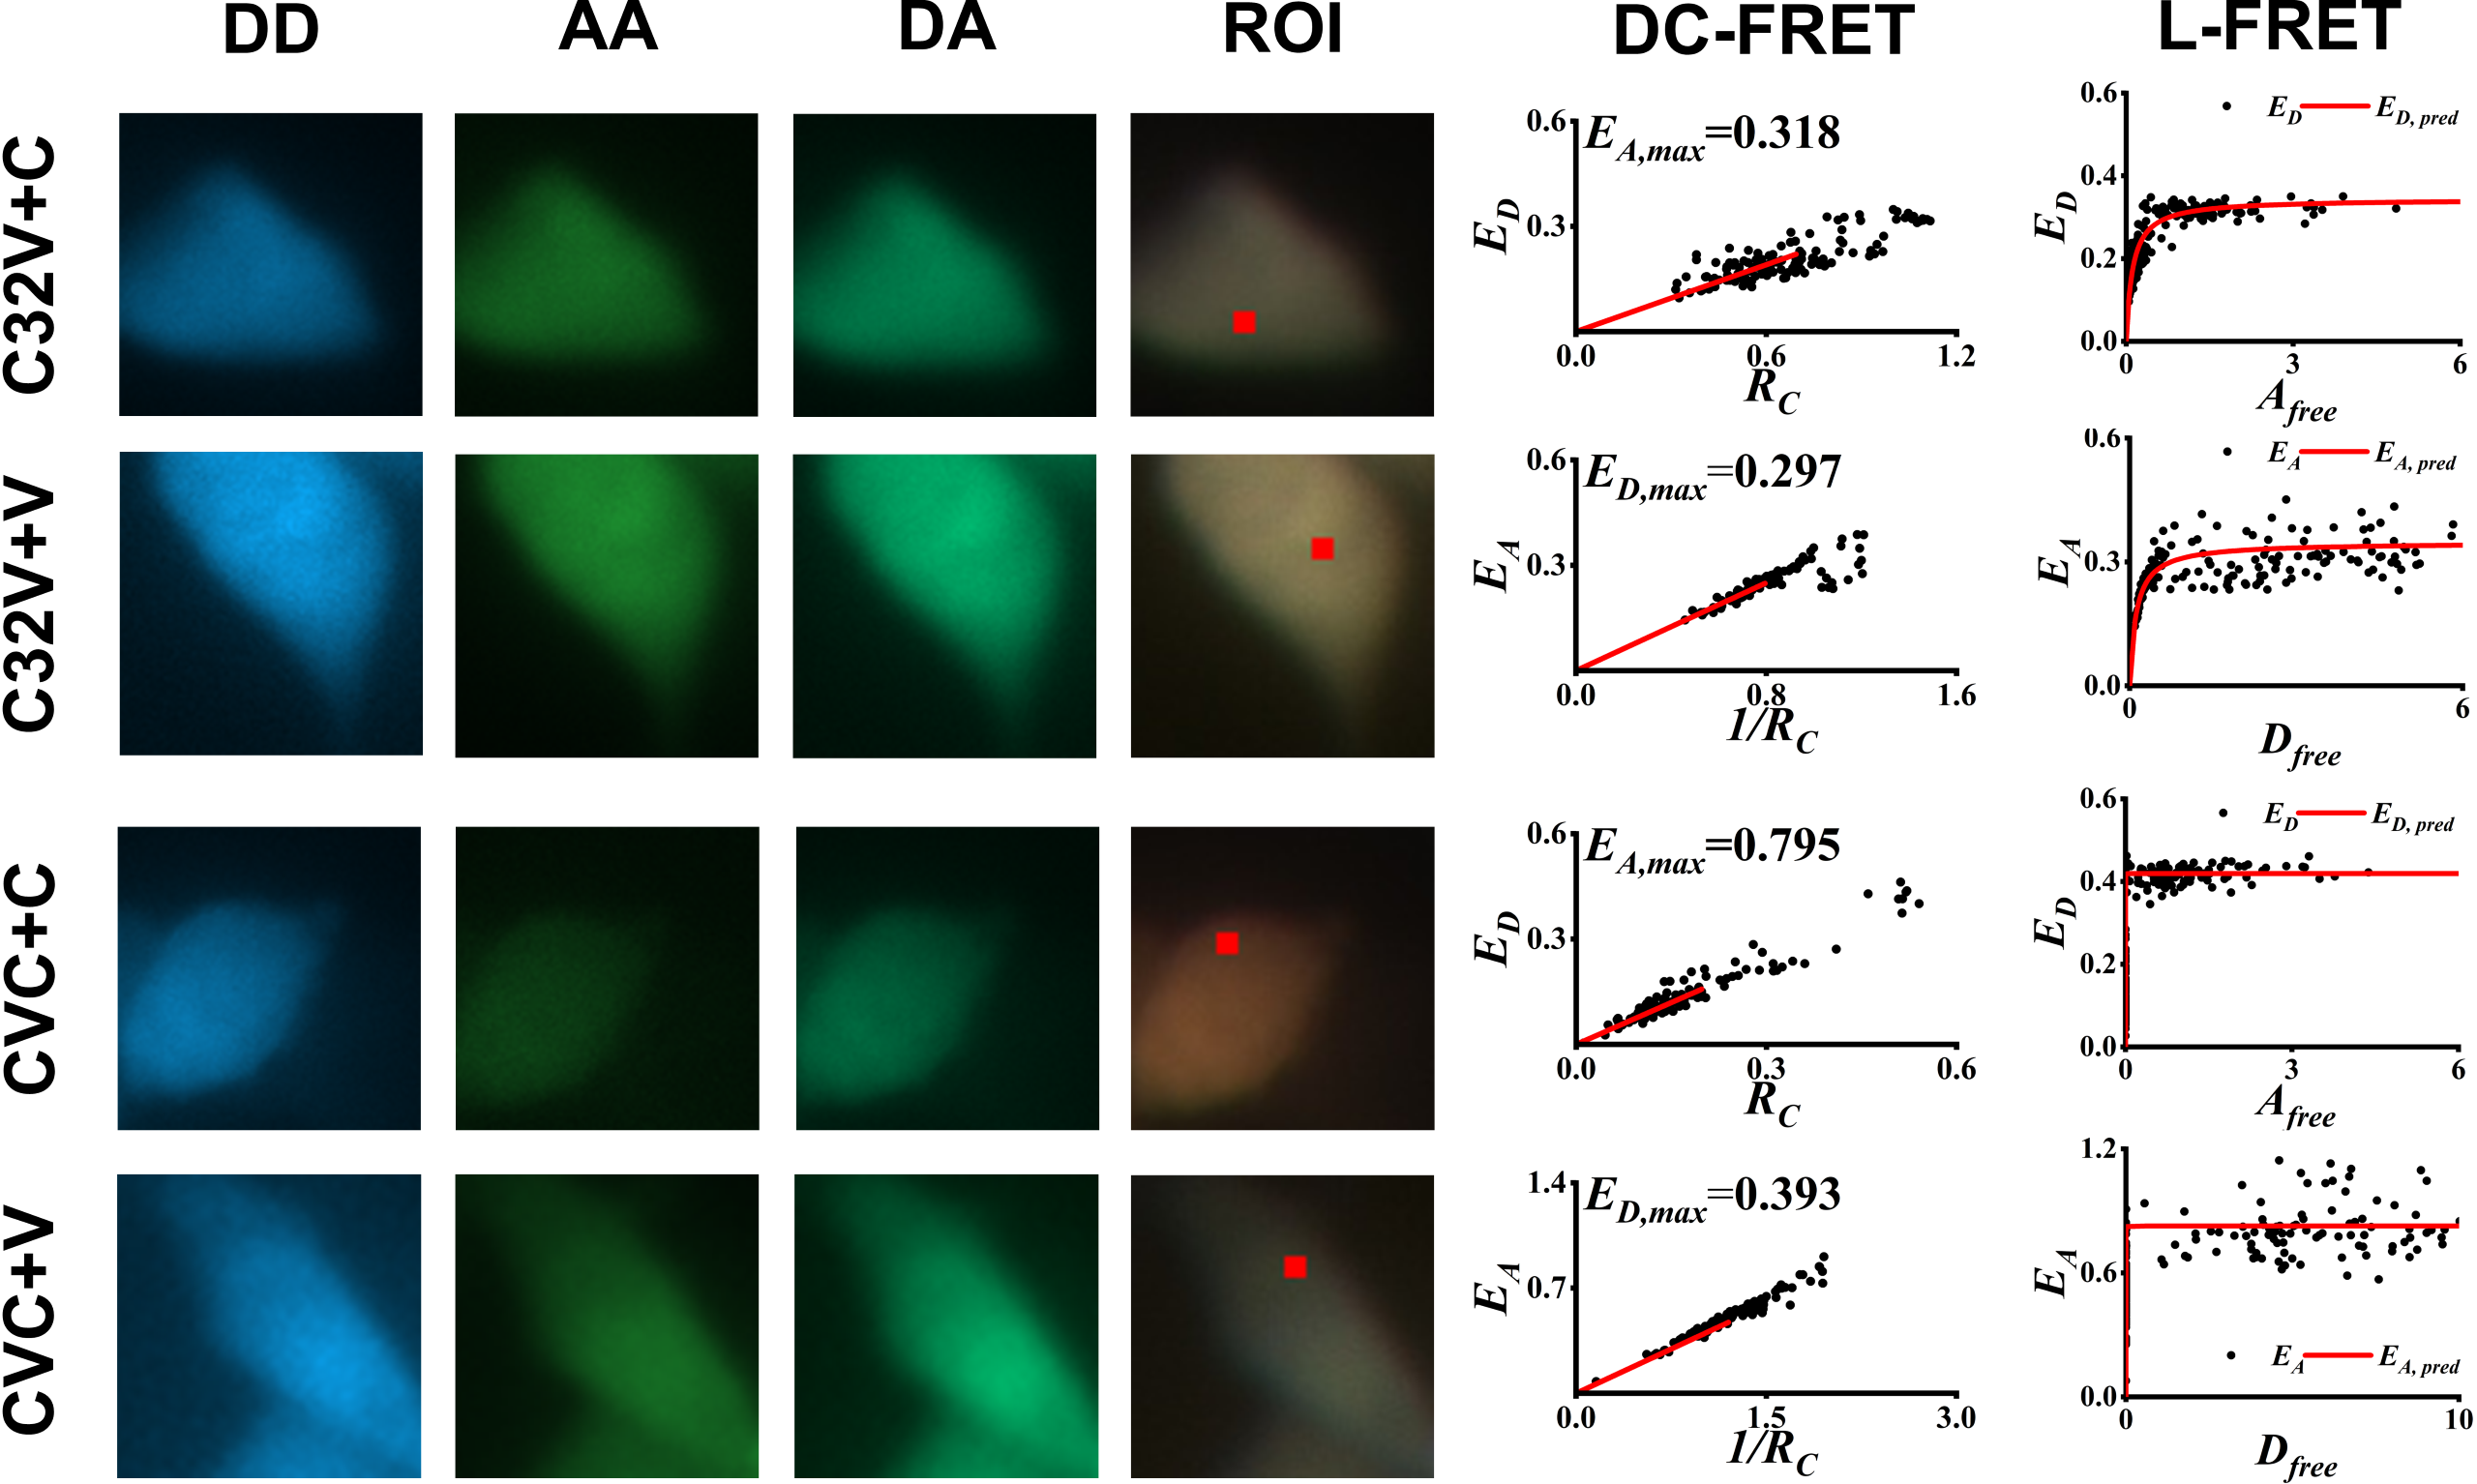
\includegraphics[width=1\linewidth]{../figures/3/验证-手动双杂交结果.drawio.png}
  \caption{Fretha手动处理的C32V和CVC的FRET双杂交分析结果}
  \label{fig:Fretha手动双杂交}
\end{figure}

DC-FRET的分析结果如表 \ref{tab:Fretha手动双杂交} 所示。
处理C32V数据时,选取$R_C$在0-0.7之间的数据用于斜率拟合$E_{A,max}$,选取$1/R_C$在0-0.8之间的数据用于斜率拟合$E_{D,max}$,测定的$E_{A,max}$为0.318,$E_{D,max}$为0.297,$n_D/n_A$为1.071;
对CVC,选取$R_C$在0-0.2之间的数据用于斜率拟合$E_{A,max}$,选取$1/R_C$在0-1.2之间的数据用于斜率拟合$E_{D,max}$,
测定的$E_{A,max}$为0.795,$E_{D,max}$为0.393,$n_D/n_A$为2.023。
L-FRET测量得到C32V的$E_{A,max}$为0.347,$E_{D,max}$为0.344,$n_D/n_A$为1.033,CVC的$E_{A,max}$为0.827,$E_{D,max}$为0.419,$n_D/n_A$为2.046。
文献报道的C32V的$E_{D,max}$为0.311,$n_D/n_A$为1,CVC的$E_{D,max}$为0.414,$n_D/n_A$为2。

使用Fretha进行DC-FRET和L-FRET的测量结果均与文献值一致,说明Fretha手动数据处理在准确度上满足预期。
\begin{table*}[htbp]
  \centering
  \caption{手动处理C32V、CVC的FRET双杂交分析结果}
  \begin{tabularx}{\linewidth}{
    >{\centering\arraybackslash}X
    >{\centering\arraybackslash}p{2.2cm}
    >{\centering\arraybackslash}p{2.2cm}
    >{\centering\arraybackslash}p{2.2cm}
    >{\centering\arraybackslash}X
    >{\centering\arraybackslash}X
    >{\centering\arraybackslash}X
    >{\centering\arraybackslash}X
    >{\centering\arraybackslash}X}
    \toprule[1.5pt]
    \multirow{2}{*}{样本} & \multicolumn{3}{c}{DC-FRET结果} & \multicolumn{3}{c}{L-FRET结果} & \multicolumn{2}{c}{文献结果} \\
     & $E_{A,max}$ & $E_{D,max}$ & ${n_D/n_A}$ & $E_{D,max}$ & $E_{D,max}$ & ${n_D/n_A}$ & $E_{D,max}$ & $n_D/n_A$\\
    \midrule
    C32V & $0.318\pm0.036$ & $0.297\pm0.018$ & $1.071\pm0.144$ & $0.347$ & $0.344$ & $1.033$ & 0.311 & 1\\
    CVC & $0.795\pm0.018$ & $0.393\pm0.023$ & $2.023\pm0.113$ & $0.827$ & $0.419$ & $2.046$ & 0.414 & 2\\
    \bottomrule[1.5pt]
    \end{tabularx}
  \label{tab:Fretha手动双杂交}
\end{table*}

\section{Fretha软件测试}
\subsection{成像参数设置模块测试}
成像参数设置是软件的核心功能之一,直接影响到数据处理结果的准确性。
本测试旨在验证软件成像参数设置功能的正确性和灵活性,确保软件能够及时准确响应参数的更新设置。

测试时,通过界面操作更新参数,分别用表 \ref{tab:lurs_imaging_params} CV成像参数和CY参数处理单转标准质粒C32V和C4Y样本,进行E-FRET分析计算结果$E_D$和$R_C$。、将参数和数据匹配的实验组记为正面组,将参数不匹配数据的组别记为反面组,测试结果如表 \ref{表:测试参数更新} 所示。

\begin{table}[htbp]
  \centering
  \caption{切换参数测量C4Y和C32V质粒E-FRET测量结果}
  \begin{tabular}{ccccc}
  \toprule[1.5pt]
  实验组 & 参数 & 样本 & $E_D$ & $R_C$ \\
  \midrule
  \multirow{2}{*}{正面} & CV & C32V & $0.299\pm0.022$ & $0.981\pm0.113$ \\
  & CY & C4Y & $0.307\pm0.040$ & $0.994\pm0.096$ \\
  \multirow{2}{*}{反面} & CY & C32V & $0.382\pm0.054$ & $0.821\pm0.093$ \\
  & CV & C4Y & $0.221\pm0.037$ & $1.313\pm0.135$ \\
  \bottomrule[1.5pt]
  \end{tabular}
  \label{表:测试参数更新}
\end{table}

正面组的测量结果中,C32V的$E_D$为$0.299\pm0.022$,$R_C$为$0.981\pm0.113$,C4Y的$E_D$为$0.307\pm0.040$,$R_C$为$0.994\pm0.096$,均与文献值一致。
反面组的测量结果中,C32V的$E_D$为$0.382\pm0.054$,$R_C$为$0.821\pm0.093$,C4Y的$E_D$为$0.221\pm0.037$,$R_C$为$1.313\pm0.135$,与文献值存在较大偏差。
说明参数Fretha后台能够及时使用更新后的参数进行计算。

经过对界面和计算结果的检查和测试,成像参数设置模块的界面和功能均符合预期,软件界面和后台内存中的参数均能准备设置更新。

\subsection{数据检验模块测试}
如 \ref{sec:数据检验模块} 节所述,数据检验模块用于检查数据的完整性和安全性,防止非法数据对软件运行造成不可预测的影响。
本测试旨在验证软件数据检验模块的有效性,并检查软件对于异常数据的识别能力和隔离能力。

测试时,使用Fretha分别尝试打开FRET标准数据、FRET缺失数据、非FRET数据、空数据、异常数据,检查软件的数据检验模块的反应。
具体测试内容和结果如表 \ref{tab:测试数据完备性} 所示。

\begin{table*}[htbp]
  \centering
  \caption{Fretha数据检验模块测试结果 }
  \begin{tabular}{cccccc}
  \toprule[1.5pt]
  测试数据 & 视野文件夹内容 & 可打开 & 可计算 & 识别类别 & 是否符合预期\\
  \midrule

  \multirow{3}{*}{FRET标准数据} &
  \begin{tabular}[t]{@{}l@{}}
    DD.tif \\
    DA.tif \\
    AA.tif \\
  \end{tabular} &
  \multirow{3}{*}{\ding{51}} &
  \multirow{3}{*}{\ding{51}} &
  \multirow{3}{*}{FRET} &
  \multirow{3}{*}{\ding{51}}\\

  \multirow{2}{*}{FRET缺失数据} &
  \begin{tabular}[t]{@{}l@{}}
    DD.tif \\
    DA.tif \\
  \end{tabular} &
  \multirow{2}{*}{\ding{51}} & 
  \multirow{2}{*}{\ding{55}} &
  \multirow{2}{*}{Unknown} &
  \multirow{2}{*}{\ding{51}} \\

  \multirow{2}{*}{非FRET数据} &
  \begin{tabular}[t]{@{}l@{}}
    D.tif \\
    A.tif \\
  \end{tabular} &
  \multirow{2}{*}{\ding{51}} &
  \multirow{2}{*}{\ding{55}} &
  \multirow{2}{*}{Unknown} &
  \multirow{2}{*}{\ding{51}} \\

  空数据 &
  空 &
  \ding{55} &
  \ding{55} &
  Unknown &
  \ding{51} \\

  \multirow{3}{*}{损坏数据} &
  \begin{tabular}[t]{@{}c@{}}
    DD.tif(损坏) \\
    DA.tif \\
    AA.tif \\
  \end{tabular} &
  \multirow{3}{*}{\ding{51}} &
  \multirow{3}{*}{\ding{55}} &
  \multirow{3}{*}{Unknown} &
  \multirow{3}{*}{\ding{51}} \\
  
  \bottomrule[1.5pt]
  \end{tabular}
  \label{tab:测试数据完备性}
\end{table*}

结果表明,对于正常数据(FRET标准数据),数据检验模块能够正确识别数据类型,并且能够成功打开和计算数据,符合预期。
对于视野子文件夹中存在缺失数据、非FRET数据、空数据和损坏数据等情况,Fretha能够打开并显示在视野区,但无法打开或者参与自动计算,并且会被正常识别为“Unknown”类别以提醒用户该视野处于不可计算的状态。
点击“自动圈点”后,发现自动算法也能够成功忽略被识别为“Unknown”类别的视野,不会对其进行计算。
这些结果均符合预期,说明软件数据检验模块的功能正常,能够有效识别和阻止异常数据的计算。

\subsection{FRET图像处理模块测试}

FRET图像处理模块能够帮助用户进行FRET双杂交分析数据处理,其功能如 \ref{sec:FRET图像处理模块} 节所述。
在测试时,我们主要测试FRET图像处理的视图增强、ROI编辑和ROI状态栏更新功能,以验证软件的功能是否符合预期。

首先测试FRET视图增强功能,分别切换表 \ref{tab:fretha_viewtype_list} 中的视图类型,查看视图增强的效果,过程中的软件界面和增强视图的截图如图 \ref{fig:视图测试} 所示。
结果表明,软件能够正确显示不同类型的视图,并且视图增强的效果明显,提高了用户在圈选ROI时的针对性和准确性。

\begin{figure*}[!hbt]
  \centering
  \includegraphics[width=0.9\linewidth]{../figures/3/测试-视图切换.drawio.png}
  \caption{Fretha图像处理视图切换测试结果}
  \label{fig:视图测试}
\end{figure*}

然后测试ROI绘制功能。
ROI编辑功能根据鼠标与ROI边框的位置关系,显示不同的鼠标样式。
分别移动鼠标位置到ROI内部、边框和外部的,观察鼠标的样式和按下时对应的功能。
测试结果如表 \ref{tab:ROI鼠标样式} 所示,表明软件能够正确显示不同的鼠标样式,且在不同位置对应的功能正确,响应迅速,保证了ROI绘制的操作体验。
\begin{table}
  \centering
  \caption{ROI绘制功能测试结果}
  \begin{tabular}{cccc}
    \toprule[1.5pt]
    鼠标位置 & 鼠标样式 & 按下效果 & 是否符合预期\\
    \midrule
    ROI内部 & 手型 & 移动ROI & \ding{51}\\
    ROI左边框 & 水平箭头 & 调整ROI宽度 & \ding{51} \\
    ROI右边框 & 水平箭头 & 调整ROI宽度 & \ding{51} \\
    ROI上边框 & 垂直箭头 & 调整ROI高度 & \ding{51} \\
    ROI下边框 & 垂直箭头 & 调整ROI高度 & \ding{51} \\
    ROI外部 & 十字形 & 新建ROI & \ding{51} \\
    \bottomrule[1.5pt]
  \end{tabular}
  \label{tab:ROI鼠标样式}
\end{table}

最后测试ROI状态栏的更新。
ROI状态栏上的数据更新发生在ROI被绘制更新以及视野切换时,因此通过更新ROI和切换视野两种操作来测试ROI状态栏信息的更新情况,结果如表 \ref{tab:ROI状态栏测试} 所示。
\begin{table}
  \centering
  \caption{ROI状态栏功能测试结果}
  \begin{tabular}{cccc}
    \toprule[1.5pt]
    \multirow{2}{*}{测试目标} & \multicolumn{2}{c}{ 测试结果} & \multirow{2}{*}{ 是否符合预期} \\
    & 更新ROI结果 & 切换视野结果 & \\
    \midrule
    DD通道信号 & 数据更新 & 重置为0 & \ding{51} \\
    DA通道信号 & 数据更新 & 重置为0 & \ding{51} \\
    AA通道信号 & 数据更新 & 重置为0 & \ding{51} \\
    DD通道SBR & 数据更新 & 重置为0 & \ding{51} \\
    DA通道SBR & 数据更新 & 重置为0 & \ding{51} \\
    AA通道SBR & 数据更新 & 重置为0 & \ding{51} \\
    DD通道背景 & 保持不变 & 数据更新 & \ding{51} \\
    DA通道背景 & 保持不变 & 数据更新 & \ding{51} \\
    AA通道背景 & 保持不变 & 数据更新 & \ding{51} \\
    $F_C$ & 数据更新 & 重置为0 & \ding{51} \\
    $E_D$ & 数据更新 & 重置为0 & \ding{51} \\
    $R_C$ & 数据更新 & 重置为0 & \ding{51} \\
    \bottomrule[1.5pt]
  \end{tabular}
  \label{tab:ROI状态栏测试}
\end{table}

上述测试结果表明,FRET图像处理的视图增强、ROI绘制和ROI状态栏更新功能均符合预期,软件能够正确显示不同类型的视图,辅助用户更好完成FRET双杂交分析图像处理工作。

\subsection{数据管理模块测试}

数据管理模块能够管理和组织数据区记录的数据,包括数据导入、数据导出、数据保存、数据计算等功能,如 \ref{sec:数据管理模块} 节所述。本节重点关注验证数据导入、数据导出和功能。
测试时的具体步骤如下:
\begin{enumerate}
  \item 使用导出数据功能导出圈点信息,检查文件生成和内容是否正确;
  \item 清空数据区,然后使用导入数据功能导入Fretha圈点数据(CSV),检查数据是否正确导入;
  \item 将导出文件另存为其他格式(XLSX),尝试导入XLSX文件,检查数据是否正确导入;
  \item 将另一组数据集生成的CSV文件导入,检查数据是否正确导入。
\end{enumerate}

测试结果如表 \ref{tab:数据管理模块测试结果} 所示。
当导入CSV格式的Fretha圈点数据,软件能够成功导入数据,数据准确无误;
导入XLSX格式的数据时,软件无法导入;
当导入不匹配Fretha数据时,软件能够检测到数据不匹配,终止导入;
导出功能能够成功导出Fretha圈点数据,数据准确无误。
添加数据和删除数据功能均工作正常,且通过鼠标和快捷键均可以快速添加和删除数据。

\begin{table}[hbtp]
  \centering
  \caption{数据管理模块测试结果}
  \begin{tabular}{p{1.5cm} l c c} % 自定义各列宽度
    \toprule[1.5pt]
    {测试目标} & {测试内容} & {测试结果} & {是否符合预期} \\
    \midrule
    \multirow{2}{*}{清空数据} & 点击“清空数据”按钮 & 成功清空 & \ding{51} \\
                             & 按下快捷键“C” & 成功清空 & \ding{51} \\
    筛选数据 & 点击“筛选数据”按钮 & 成功筛选 & \ding{51} \\
    \multirow{3}{*}{导入数据} & 导入Fretha圈点数据(CSV) & 成功导入 & \ding{51} \\
     & 导入其他表格类型数据(XLSX) & 无法导入 & \ding{51} \\
     & 导入不匹配Fretha数据(CSV) & 无法导入 & \ding{51} \\
    导出数据 & 导出Fretha圈点数据(CSV) & 成功导出 & \ding{51} \\
    \multirow{2}{*}{添加数据} & 点击“添加数据”按钮 & 成功添加 & \ding{51} \\
     & 按下快捷键“A” & 成功添加 & \ding{51} \\
    \multirow{2}{*}{删除数据} & 点击“删除数据”按钮 & 成功删除 & \ding{51} \\ 
     & 按下快捷键“D” & 成功删除 & \ding{51} \\
    开始计算 & 开始结算功能和跳转 & 页面跳转,结果准确 & \ding{51} \\

    \bottomrule[1.5pt]
  \end{tabular}
  \label{tab:数据管理模块测试结果}
\end{table}

\subsection{结果可视化模块测试}

结果可视化和保存模块能够帮助用户查看和保存数据处理结果,包括视图选择、图表结果、结果保存等,如 \ref{sec:结果可视化模块} 节所述。
本节对上述功能进行测试时,重点关注两种视图的显示、参数的更新和结果的保存功能。
\begin{figure}[htbp]
  \centering
  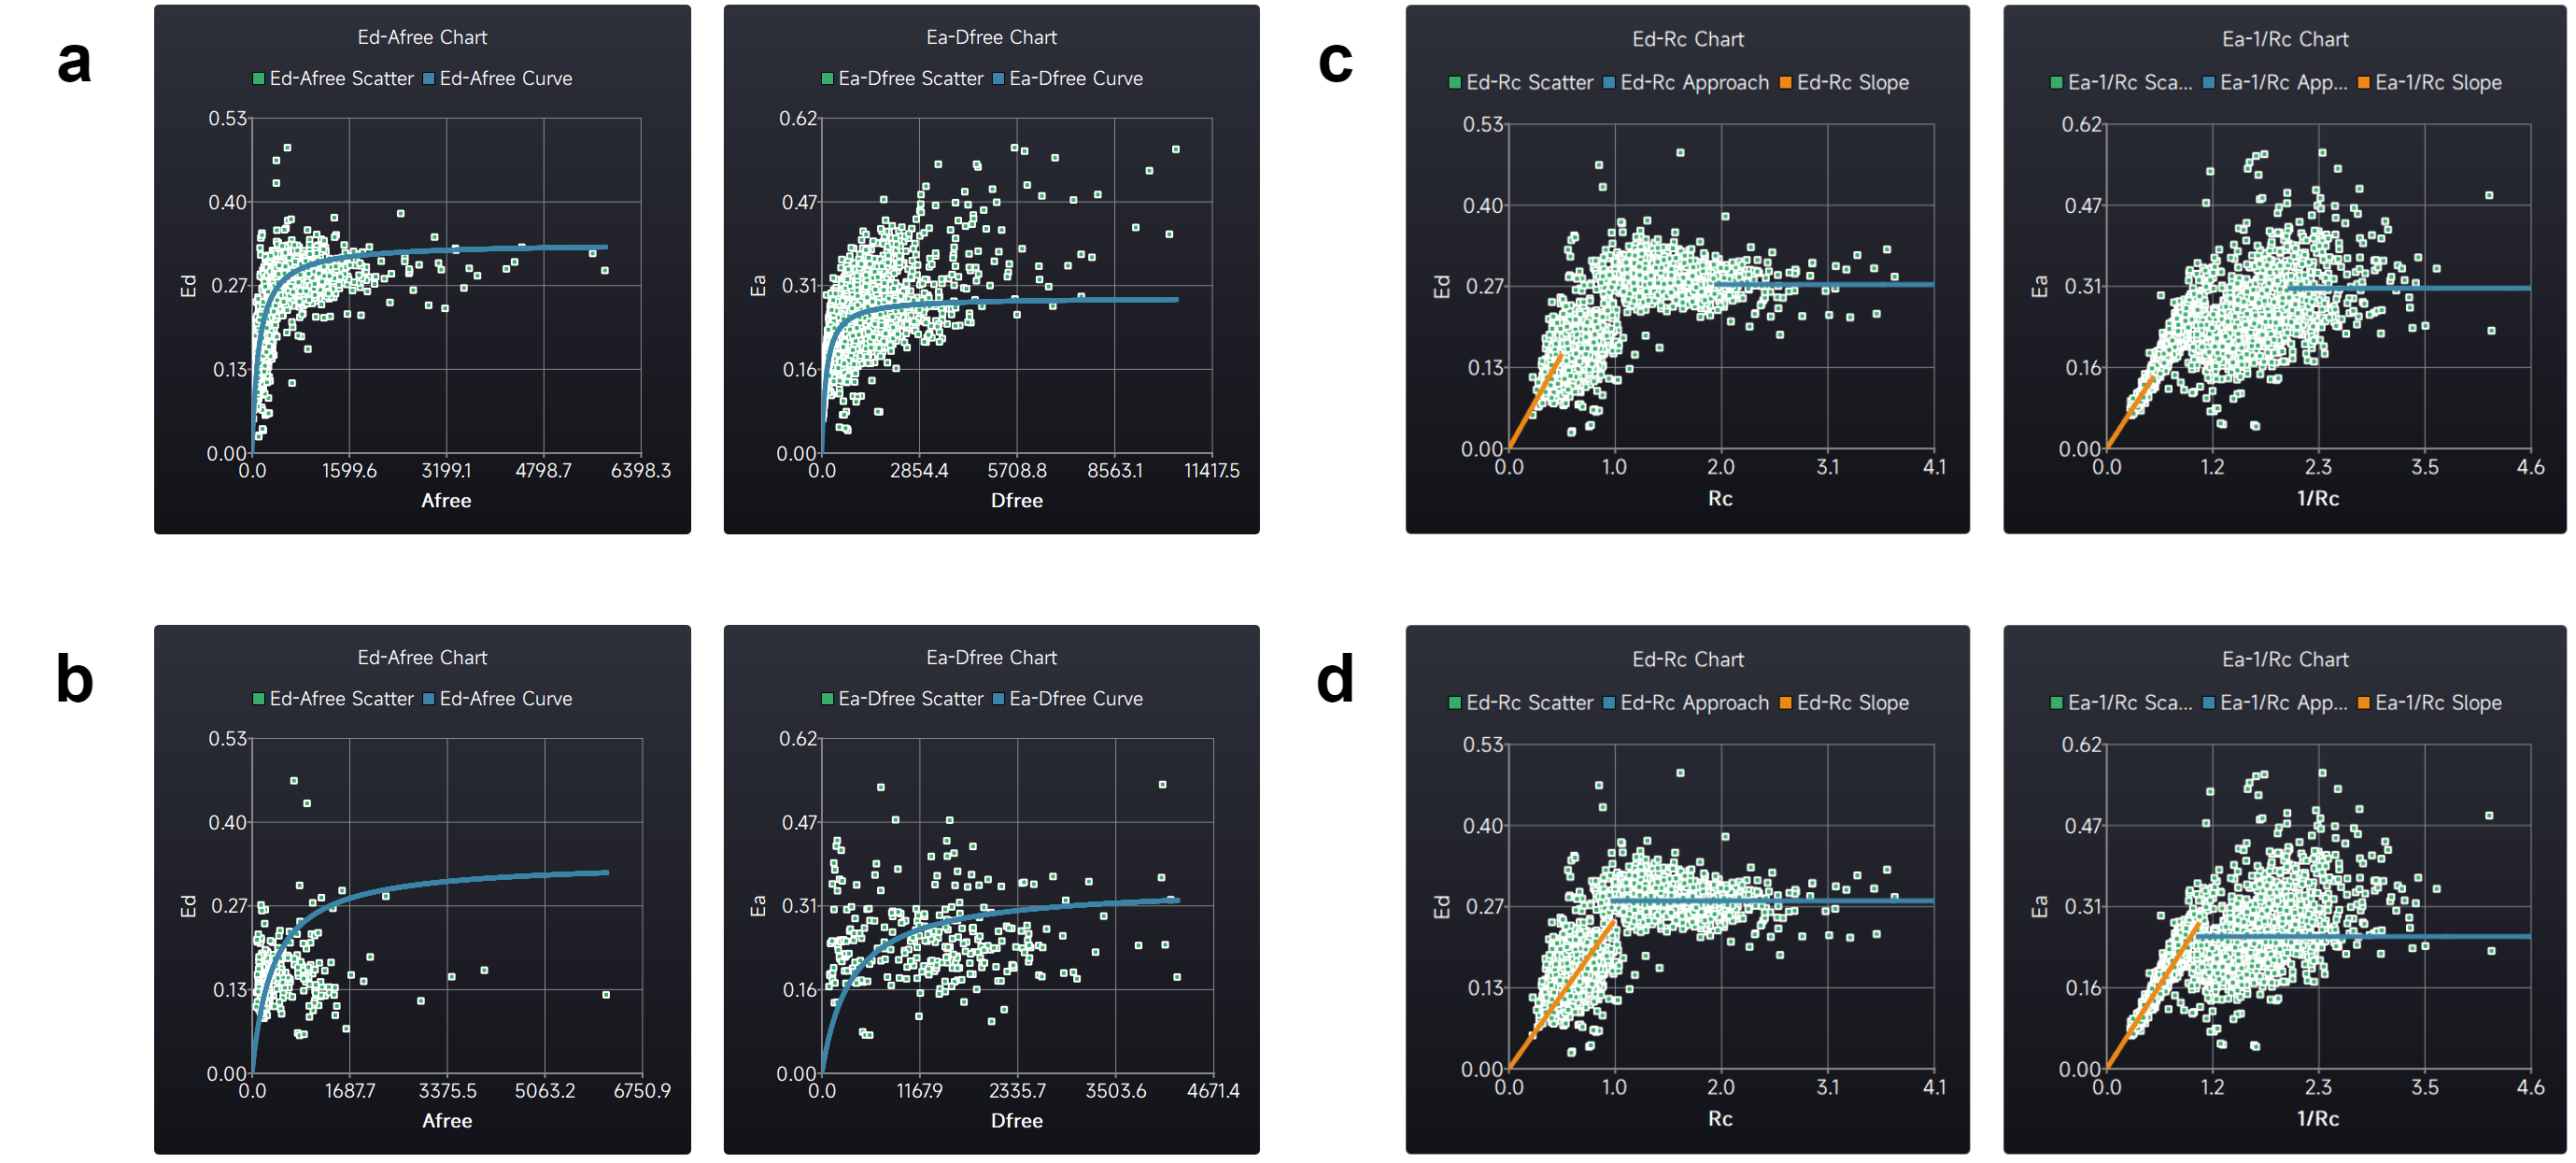
\includegraphics[width=1\linewidth]{../figures/3/测试-结果可视化.drawio.png}
  \caption[Fretha L-FRET视图测试结果]{Fretha L-FRET视图和DC-FRET视图。图a为标准L-FRET视图;图b为应用BIN数据分箱后的L-FRET视图;图c为设置线性拟合的$R_C$数据范围为$(0,0.5)$,均值拟合的$R_C$范围为$(2,10)$时的DC-FRET视图;图d设置线性拟合的$1/R_C$数据范围为$(0,1)$,均值拟合的$1/R_C$范围为$(1,10)$。}
  \label{fig:L-FRET视图测试}
\end{figure}

测试L-FRET视图和BIN数据分箱功能,测试结果如图 \ref{fig:L-FRET视图测试} 中图a和图b所示。
L-FRET显示出良好的拟合效果,散点与趋势线符合预期。
测试所用的BIN参数为对$R_C$在$(0,5)$之间的数据按照0.01的步长进行分组并计算平均值,结果显示BIN参数更新后的L-FRET视图散点数明显减少,且趋势线有所变化。
测试DC-FRET视图中调整线性拟合的数据范围参数设置功能时,首先设置线性拟合的$R_C$数据范围为$(0,0.5)$,均值拟合的$R_C$范围为$(2,10)$,然后设置线性拟合的$1/R_C$数据范围为$(0,1)$,均值拟合的$1/R_C$范围为$(1,10)$,观察图表中的趋势线和散点图更新。
测试结果如图 \ref{fig:L-FRET视图测试} 中图C和图d所示,当扩大拟合数据的范围后,可以观察到趋势线的更新,斜率拟合段和均值拟合段均延伸至$R_C$为1的位置。

测试结果可视化的结果保存功能,检查目标目录下生成的文件,发现存在两个CSV文件和四张散点趋势线图,符合表 \ref{tab:fretha_result_list} 设计,软件能够正确生成结果文件,且图片和表格文件的可以正常打开。

综合测试结果表明,Fretha结果可视化模块的功能正常,能够正确显示和保存数据处理结果,为用户提供了直观的数据分析和保存功能。

\section{Fretha可靠性测试}
可靠性测试旨在评估 Fretha 软件在长时间运行、高负载或异常操作下的可靠性。测试包括:
\begin{enumerate}
  \item 压力测试:同时加载 10 个大型 FRET 数据集(每个数据集包含 50 个视野),连续执行参数设置、图像处理和结果计算操作,监测软件是否出现崩溃或内存泄漏;
  \item 长时间运行测试:保持软件连续运行 48 小时,期间每隔8小时进行数据导入、数据计算和保存,然后清空数据。记录软件内存占用情况,检测软件是否存在内存泄露;
  \item 异常操作测试:快速重复进行参数切换、数据导入导出、ROI 编辑等操作,模拟用户高频使用场景,观察软件的响应稳定性。
\end{enumerate}

\begin{figure}[tp]
  \centering
  \includegraphics[width=0.6\linewidth]{../figures/3/测试-48小时内存波动.drawio.png}
  \caption{Fretha软件48小时运行内存占用监测}
  \label{fig:48小时内存变化}
\end{figure}

测试结果如表 \ref{tab:稳定性测试} 所示。
\begin{table}[htbp]
  \centering
  \caption{Fretha 软件可靠性测试结果}
  \label{tab:稳定性测试}
  \begin{tabularx}{\linewidth}{lXX}
  \toprule[1.5pt]
  {测试类型} & {测试方法} & {测试结果} \\
  \midrule 
  \multirow{3}{*}{压力测试} 
    & \multirow{3}{\linewidth}{连续处理 10 个包含 50 个视野的大型数据,监测软件是否出现崩溃或内存泄漏。} 
    & - 处理 10 个数据集总耗时:42.5 分钟 \\
    &                                                                                
    & - 内存峰值占用:1.1 GB(稳定无泄漏) \\
    &                                                                                
    & - 操作成功率:100\% \\
  % \midrule % 测试类型分隔线
  \multirow{4}{*}{长时间运行测试} 
    & \multirow{4}{\linewidth}{保持软件连续运行 48 小时,每8小时执行数据导入$\rightarrow$数据计算$\rightarrow$结果保存$\rightarrow$数据清除,记录 CPU 和内存占用情况。} 
    & - CPU 使用率:22 - 25\%(波动<3\%) \\
    &                                                                                
    & - 内存占用:550 - 900 MB(无持续增长) \\
    &                                                                                
    & - 数据导出成功率:100\% \\
  % \midrule % 测试类型分隔线
  \multirow{3}{*}{异常操作测试} 
    & \multirow{3}{\linewidth}{快速重复进行参数切换、数据导入导出、ROI 编辑等操作,模拟用户高频使用场景,观察软件的响应稳定性。} 
    & - 每秒操作次数:15-20 次/秒 \\
    &                                                                                
    & - 平均响应时间:0.3-0.5 秒 \\
    &                                                                                
    & - 未出现卡顿或界面冻结 \\
  \bottomrule[1.5pt]
  \end{tabularx}
\end{table}
首先,Fretha 在压力测试下仍能稳定处理数据,连续处理了10个大型的数据过程中未出现崩溃或内存溢出。
其次,长时间运行中的内存占用监测如图 \ref{fig:48小时内存变化} 所示,期间每次清空数据后内存占用没有显著增加,且软件功能运行正常;高频操作下软件响应迅速,未出现卡顿或错误。
这些结果证明 Fretha 具有良好的稳定性,能够满足科研和工业场景的长时间、高负载使用需求。

\section{本章小结}
本章应用Fretha进行验证实验,并对每个功能模块进行单独测试,验证了Fretha数据处理的准确性、可靠性和易用性。
首先,通过标准质粒的E-FRET分析和$3^3$-FRET分析,在核心FRET指标$E_A$、$E_D$和$R_C$的测定中,Fretha计算C4Y、C10Y、C40Y和C80Y的结果与文献值的平均误差不超过3.9\%,验证了Fretha数据处理计算FRET效率的准确性,确保为FRET双杂交分析提供准确的FRET效率等数值。
然后,在FRET双杂交模型质粒C32V和CVC的分析中,Fretha计算出在C32V中Cerulean和Venus结合的化学计量比例$n_D/n_A$为1.071,在CVC中为2.023,成功检测到两种质粒中化学计量比的差异。
接着,本章针对各功能模块进行了单独测试,包括成像参数设置模块、数据检验模块、FRET图像处理模块、数据管理模块、结果可视化模块。
每个模块的核心功能均通过测试,使用体验良好,验证了软件的功能完整和易用性。
最后,本章在可靠性测试中进一步验证了Fretha在长时间运行、高负载和高频操作下的可靠性,未出现崩溃或性能下降的情况。
综合测试结果表明,Fretha软件测量准确、功能完善、可靠性良好,能够满足复杂科研和实际应用的需求。